% !TeX program = lualatex
% ================================================================
% Portuguese Parallel Text Version of RecurringDecimalsToFractions
%
% Generated by the server using the following settings:
%
%   language            Portuguese (por)
%   text direction      left to right
%   font                Noto Serif
%   fallback font       Noto Serif
%   built from          latex/worksheets/fractions/recurringDecimalsToFractions.tex
%   vocabulary key      latex/worksheets/fractions/recurringDecimalsToFractions/L2/por/recurringDecimalsToFractions_portugueseKey.tex
%   tier 3 vocabulary   green   RGB 0 128 0
%   English text        black   RGB 0 0 0
%   Portuguese text     purple  RGB 112 48 160
%   layout macros       version 3
%
% Please don't edit any information in this comment block - the server
% compares it against the current settings and rebuilds this file when
% they differ, so changes here would be overwritten. However, feel free
% to make updates to the LaTeX below if you want to edit it.
% ================================================================

\documentclass[12pt,a4paper]{article}
% ================================================================
% Copied from the English sheet this was translated from, so that
% anything it sets up for itself still works here
% ================================================================
\usepackage[a4paper,top=12mm,bottom=14mm,left=15mm,right=15mm]{geometry}
\usepackage[T1]{fontenc}
\usepackage{amsmath}
\usepackage{amssymb}
\usepackage{enumitem}
\usepackage{multicol}
\usepackage{tikz}
\usepackage[most]{tcolorbox}
\usetikzlibrary{decorations.pathreplacing,arrows.meta}

% ================================================================
% Recurring decimals to fractions.
%
% An extension sheet for the top end of a middle ability Year 9
% class, designed to be worked through alone: every method is
% introduced by a worked example, practised once with the steps
% written out, and then practised without them. Answers are on the
% last page so that pupils can check each part before going on.
%
% The sheet is written on, so it is set with open leading and wide
% list separation, and every question is followed by a working area
% sized to fill the rest of its page. The \newpage commands in the
% body are placed so that no question is ever split across the fold;
% because of them a part may run to more than one page.
% ================================================================

\pagestyle{empty}
\linespread{1.2}\selectfont
\setlength{\parskip}{5pt}
\renewcommand{\arraystretch}{1.35}
\setlist[enumerate,1]{label=\textbf{Q\arabic*.}, leftmargin=*, itemsep=12pt, topsep=8pt, parsep=4pt}
\setlist[enumerate,2]{label=(\alph*), leftmargin=*, itemsep=8pt, topsep=5pt, parsep=3pt}
\setlength{\multicolsep}{8pt}
\setlength{\parindent}{0pt}

\newcommand{\ansline}[1][2.2cm]{\underline{\hspace{#1}}}

% A worked example: the method shown in full before it is practised.
\newtcolorbox{wex}[1]{colback=blue!4,colframe=blue!45!black,boxrule=0.6pt,
  left=6pt,right=6pt,top=4pt,bottom=5pt,
  title={\bfseries\small Worked example: #1},fonttitle=\small,
  toptitle=1pt,bottomtitle=1pt}

% The idea a section is built on, stated once and boxed.
\newtcolorbox{keyidea}{colback=orange!7,colframe=orange!60!black,boxrule=0.6pt,
  left=6pt,right=6pt,top=4pt,bottom=4pt}

% The section headings, kept tight so the parts do not eat the page.
\newcommand{\heading}[1]{%
  \vspace{2pt}
  {\color{blue!45!black}\rule{\linewidth}{1pt}}\\[1pt]
  {\large\bfseries #1}\\[-6pt]
  {\color{blue!45!black}\rule{\linewidth}{0.4pt}}
  \vspace{2pt}}
\newcommand{\parttitle}[2]{\heading{Part #1: #2}}

% ----------------------------------------------------------------
% One line of a subtraction diagram. Every row puts its decimal
% point at the same x, so that recurring tails which really are
% identical end up in the same columns on the page.
% \drow{<y>}{<label>}{<digits before the point>}{<digits after>}
\newcommand{\drow}[4]{%
  \node[anchor=east,font=\small] at (-1.25,#1) {#2};
  \node[anchor=east,font=\small] at (-0.12,#1) {#3};
  \node[font=\small] at (0,#1) {.};
  \foreach \d [count=\i from 0] in {#4}
    {\node[font=\small] at ({0.34+\i*0.34},#1) {\d};}%
}
% The band of columns from digit #1 to digit #2, used to shade a tail.
\newcommand{\tailbox}[4]{%
  ({0.34+#1*0.34-0.17},#3) rectangle ({0.34+#2*0.34+0.17},#4)}
% The same row as \drow, but with a writing line in each digit column so that
% a pupil fills the row in. #4 is how many columns to draw before the dots.
% \drowgap{<y>}{<label>}{<before the point>}{<number of columns>}
\newcommand{\drowgap}[4]{%
  \node[anchor=east,font=\small] at (-1.25,#1) {#2};
  \node[anchor=east,font=\small] at (-0.12,#1) {#3};
  \node[font=\small] at (0,#1) {.};
  \foreach \i in {1,...,#4}
    {\draw[gray!60] ({0.34+(\i-1)*0.34-0.13},{#1-0.16}) --
                    ({0.34+(\i-1)*0.34+0.13},{#1-0.16});}
  \node[font=\small] at ({0.34+#4*0.34},#1) {$\ldots$};%
}
% Solving by dividing both sides: the equation before above the equation
% after, with a curved arrow down each side carrying the division. Both
% arrows bend outwards, so neither crosses the equation.
% \divideboth{<lhs>}{<rhs>}{<new lhs>}{<new rhs>}{<divisor>}
\newcommand{\divideboth}[5]{%
  \begin{tikzpicture}
    \node (tl) at (0,0)     {$#1$};
    \node       at (0.7,0)  {$=$};
    \node (tr) at (1.5,0)   {$#2$};
    \node (bl) at (0,-1.5)  {$#3$};
    \node       at (0.7,-1.5) {$=$};
    \node (br) at (1.5,-1.5) {$#4$};
    \draw[-{Stealth[length=2mm]},blue!45!black] (tl) to[bend right=65]
      node[left=1pt,font=\scriptsize]{$\div\,#5$} (bl);
    \draw[-{Stealth[length=2mm]},blue!45!black] (tr) to[bend left=65]
      node[right=1pt,font=\scriptsize]{$\div\,#5$} (br);
  \end{tikzpicture}%
}

% Characters this language's font has not got are borrowed from another,
% rather than being silently dropped - see docs/translated-sheet-latex.md
\directlua{%
  if luaotfload and luaotfload.add_fallback then
    luaotfload.add_fallback("eallatinfallback",
      { "Noto Serif:mode=harf;" })
  else
    tex.error("this luaotfload is too old to register a fallback font")
  end
}
\usepackage[english]{babel}
\babelprovide[import]{portuguese}
\babelfont[portuguese]{rm}[Renderer=Harfbuzz, BoldFont={Noto Serif}, ItalicFont={Noto Serif}, BoldItalicFont={Noto Serif}, RawFeature={fallback=eallatinfallback}]{Noto Serif}
\babelfont[portuguese]{sf}[Renderer=Harfbuzz, BoldFont={Noto Serif}, ItalicFont={Noto Serif}, BoldItalicFont={Noto Serif}, RawFeature={fallback=eallatinfallback}]{Noto Serif}
\newcommand{\ealtext}[1]{\foreignlanguage{portuguese}{#1}}
\newcommand{\ealtextblock}[1]{{\raggedright\foreignlanguage{portuguese}{#1}\par}}
% ================================================================
% EAL layout helpers
% ================================================================
\usepackage{xcolor}

\definecolor{ealkeycolour}{RGB}{0,128,0}
\definecolor{ealenglish}{RGB}{0,0,0}
\definecolor{ealtwocolour}{RGB}{112,48,160}

\newsavebox{\ealboxen}
\newsavebox{\ealboxtr}
\newlength{\ealglosswd}
\newlength{\ealglossraise}
\setlength{\ealglossraise}{1.15em}

% a tier 3 word, in English and in translation alike
\newcommand{\ealkey}[1]{\textcolor{ealkeycolour}{#1}}
\newcommand{\ealkeytr}[1]{\textcolor{ealkeycolour}{\ealtext{#1}}}

% One translated word above one English word. Built from kernel
% primitives, never a tabular, which would break wherever the sheet
% loads array, booktabs or tabularx. The box is as wide as the wider of
% the two, so a long translation pushes its neighbours aside instead of
% overlapping them, and it claims its full height so a table row or a
% TikZ node makes room for it.
\newcommand{\ealgloss}[2]{%
  \sbox{\ealboxen}{\ealkey{#1}}%
  \sbox{\ealboxtr}{\small\textcolor{ealtwocolour}{\ealtext{#2}}}%
  \setlength{\ealglosswd}{\wd\ealboxen}%
  \ifdim\wd\ealboxtr>\ealglosswd\setlength{\ealglosswd}{\wd\ealboxtr}\fi
  \leavevmode
  \makebox[\ealglosswd][c]{%
    \makebox[0pt][c]{\usebox{\ealboxen}}%
    \makebox[0pt][c]{\raisebox{\ealglossraise}{\usebox{\ealboxtr}}}%
  }%
}

% opens up line spacing around a block of glosses, so the raised
% translations sit clear of the line above
\newenvironment{ealglossed}{\par\linespread{2.1}\selectfont\ignorespaces}{\par}

% a whole translated sentence above its English counterpart. block level,
% so it does not belong inside a tabular cell
\newcommand{\ealpara}[2]{%
  \par\addvspace{0.5\baselineskip}%
  {\color{ealtwocolour}\ealtextblock{#1}}%
  \penalty200
  {\color{ealenglish}#2\par}%
  \addvspace{0.5\baselineskip}%
}

\begin{document}

\begin{center}
  {\Large\bfseries \ealkey{Recurring Decimals} into \ealkey{Fractions}}\\[8pt]
\end{center}
\vspace{1pt}

\begin{keyidea}
\small
\ealpara{Toda \ealkeytr{dízima periódica} --- por mais longa e complicada que seja --- pode ser escrita como uma \ealkeytr{fração}. Segue os exemplos nesta folha para aprenderes a converter \ealkeytr{dízimas periódicas} em \ealkeytr{frações}.}{Every \ealkey{recurring decimal} --- however long and however complicated --- can be written as a \ealkey{fraction}. Follow the examples in this sheet to learn how to convert \ealkey{recurring decimals} to \ealkey{fractions}.}
\end{keyidea}

\parttitle{1}{Reading and writing \ealkey{recurring decimals}}

\ealpara{Quando divides um número inteiro por outro, os \ealkeytr{algarismos} depois da vírgula ou terminam, ou formam um bloco que se repete para sempre. Os blocos repetidos marcam-se com um ponto sobre o \textbf{primeiro} \ealkeytr{algarismo} e um ponto sobre o \textbf{último} \ealkeytr{algarismo}.}{When you divide one whole number by another, the \ealkey{digits} after the point either stop, or fall into a block that repeats forever. Repeating blocks are marked with a dot over the \textbf{first} \ealkey{digit} and a dot over the \textbf{last} \ealkey{digit}.}

\ealpara{O bloco que se repete; por isso escrevemo-lo $0.\dot{2}\dot{7}$.}{the block that repeats; so we write it $0.\dot{2}\dot{7}$}

\begin{center}
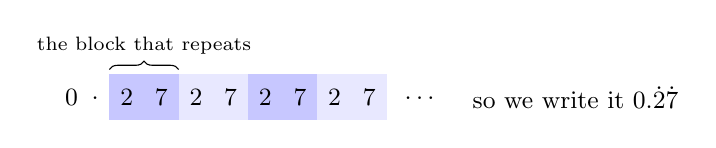
\begin{tikzpicture}[font=\small]
  \def\dgw{0.44}
  \foreach \s/\c in {0/blue!22, 2/blue!9, 4/blue!22, 6/blue!9}{
    \fill[\c] ({0.7+\s*\dgw-0.5*\dgw},-0.28) rectangle ({0.7+(\s+2)*\dgw-0.5*\dgw},0.3);}
  \node at (0,0) {$0$};
  \node at (0.3,0) {.};
  \foreach \d [count=\i from 0] in {2,7,2,7,2,7,2,7}
    {\node at ({0.7+\i*\dgw},0) {\d};}
  \node at ({0.7+8*\dgw+0.2},0) {$\ldots$};
  \draw[decorate,decoration={brace,amplitude=3pt}]
    ({0.7-0.5*\dgw},0.36) -- ({0.7+1.5*\dgw},0.36)
    node[midway,above=2pt,font=\scriptsize]{the block that repeats};
  \node[anchor=west,font=\small] at ({0.7+8*\dgw+0.75},0)
    {so we write it $0.\dot{2}\dot{7}$};
\end{tikzpicture}
\end{center}
\vspace{-4pt}

\ealpara{Assim, $0.\dot{6}=0.6666666\ldots$, \; $0.\dot{2}\dot{7}=0.2727272\ldots$, \; $0.\dot{4}0\dot{9}=0.4094094\ldots$ \; e $0.1\dot{6}=0.1666666\ldots$ --- repara que no último apenas o $6$ tem um ponto, por isso só o $6$ se repete. O $1$ encontra-se apenas na coluna das décimas e nunca regressa.}{So $0.\dot{6}=0.6666666\ldots$, \; $0.\dot{2}\dot{7}=0.2727272\ldots$, \; $0.\dot{4}0\dot{9}=0.4094094\ldots$ \; and $0.1\dot{6}=0.1666666\ldots$ --- notice that in the last one only the $6$ carries a dot, so only the $6$ repeats. The $1$ only is found in the tenths column, and never comes back.}

\vspace{2em}

\begin{enumerate}

\item \ealpara{Escreve as primeiras oito \ealkeytr{casas decimais} de cada número.}{Write out the first eight \ealkey{decimal places} of each number.}
\begin{multicols}{3}
\begin{enumerate}
  \item $0.\dot{5}=0.\ansline[2.3cm]$
  \item $0.\dot{1}\dot{8}=0.\ansline[2.3cm]$
  \item $0.3\dot{7}=0.\ansline[2.3cm]$
  \item $0.\dot{2}0\dot{6}=0.\ansline[2.3cm]$
  \item $0.4\dot{5}\dot{1}=0.\ansline[2.3cm]$
  \item $0.\dot{9}=0.\ansline[2.3cm]$
\end{enumerate}
\end{multicols}

\vspace{1em}

\item \ealpara{Escreve cada um destes usando \ealkeytr{notação com pontos}.}{Write each of these using \ealkey{dot notation}.}
\begin{multicols}{3}
\begin{enumerate}
  \item $0.8888\ldots=\ansline[1.5cm]$
  \item $0.636363\ldots=\ansline[1.5cm]$
  \item $0.24444\ldots=\ansline[1.5cm]$
  \item $0.157157\ldots=\ansline[1.5cm]$
  \item $0.91666\ldots=\ansline[1.5cm]$
  \item $0.40505\ldots=\ansline[1.5cm]$
\end{enumerate}
\end{multicols}

\vspace{1em}

\item
\begin{enumerate}
  \item \ealpara{Qual é maior, $0.\dot{4}\dot{5}$ ou $0.4\dot{5}$? Escreve ambos com seis \ealkeytr{casas decimais} para te ajudar a decidir e explica a tua resposta.}{Which is bigger, $0.\dot{4}\dot{5}$ or $0.4\dot{5}$? Write both out to six \ealkey{decimal places} to help you decide, and explain your answer.}

        \vspace{7em}
  \item \ealpara{Escreve uma \ealkeytr{dízima periódica} que esteja entre $0.\dot{3}$ e $0.\dot{4}$.}{Write down a \ealkey{recurring decimal} that lies between $0.\dot{3}$ and $0.\dot{4}$.} \ansline[3cm]
\end{enumerate}

\end{enumerate}

% \parttitle{2}{The family of nines}

% Before any algebra, here is a pattern worth knowing. Use short division to
% check the first one or two, then follow the pattern.

% \begin{enumerate}[resume]

% \item Complete the following.
% \begin{multicols}{4}
% \begin{enumerate}
%   \item $\tfrac{1}{9}=0.\dot{1}$
%   \item $\tfrac{2}{9}=\ansline[1.4cm]$
%   \item $\tfrac{4}{9}=\ansline[1.4cm]$
%   \item $\tfrac{7}{9}=\ansline[1.4cm]$
% \end{enumerate}
% \end{multicols}

% \item Now with two and three nines on the bottom.
% \begin{multicols}{3}
% \begin{enumerate}
%   \item $\tfrac{1}{99}=0.\dot{0}\dot{1}$
%   \item $\tfrac{7}{99}=\ansline[1.8cm]$
%   \item $\tfrac{14}{99}=\ansline[1.8cm]$
%   \item $\tfrac{58}{99}=\ansline[1.8cm]$
%   \item $\tfrac{1}{999}=0.\dot{0}0\dot{1}$
%   \item $\tfrac{271}{999}=\ansline[1.8cm]$
% \end{enumerate}
% \end{multicols}

% \end{enumerate}

% \begin{keyidea}
% \small
% \textbf{The nines rule.} If a block of $n$ digits repeats \emph{straight after
% the decimal point}, the fraction is that block written over $n$ nines. So
% $0.\dot{8}=\tfrac{8}{9}$, \; $0.\dot{2}\dot{7}=\tfrac{27}{99}$ \; and \;
% $0.\dot{4}0\dot{9}=\tfrac{409}{999}$. Always simplify afterwards ---
% $\tfrac{27}{99}=\tfrac{3}{11}$.
% \end{keyidea}

% \begin{enumerate}[resume]

% \item Use the nines rule. Give each answer as a fraction in its simplest form.
% \begin{multicols}{3}
% \begin{enumerate}
%   \item $0.\dot{7}$ \ansline[1.6cm]
%   \item $0.\dot{2}\dot{4}$ \ansline[1.6cm]
%   \item $0.\dot{8}\dot{1}$ \ansline[1.6cm]
%   \item $0.\dot{6}$ \ansline[1.6cm]
%   \item $0.\dot{1}3\dot{5}$ \ansline[1.6cm]
%   \item $0.\dot{4}\dot{5}$ \ansline[1.6cm]
% \end{enumerate}
% \end{multicols}

% \end{enumerate}

% The nines rule is quick, but it only works when the repeating block starts
% immediately after the point --- it is no use at all on $0.1\dot{6}$ --- and it
% does not explain \emph{why} the nines appear. For both of those we need
% algebra, and that is the rest of the sheet.

\newpage

\parttitle{2}{Finding \ealkey{fractions} from \ealkey{recurring decimals}}

\ealpara{O truque é encontrar dois números cujas caudas periódicas sejam \textbf{exatamente iguais} e, em seguida, subtrair um do outro. As caudas cancelam-se e o que resta não tem quaisquer decimais.}{The trick is to find two numbers whose recurring tails are \textbf{exactly the same}, and then subtract one from the other. The tails cancel, and what is left has no decimals in it at all.}

\ealpara{Para isso, temos de usar uma \ealkeytr{variável} \textbf{algébrica}, à qual chamaremos $x$. $x$ representa a \ealkeytr{dízima periódica} que estamos a tentar converter numa \ealkeytr{fração}.}{To do this we have to use an \textbf{algebraic \ealkey{variable}}, which we will call $x$. $x$ stands for the \ealkey{recurring decimal} we are trying to convert to a \ealkey{fraction}.}

\ealpara{Converter $0.\dot{4}$ numa \ealkeytr{fração}}{turn $0.\dot{4}$ into a \ealkey{fraction}}
\begin{wex}{}
\small
\ealpara{Passo 1 --- introduz $x$. Escrevemos $x=0.\dot{4}$, portanto $x=0.4444\ldots$}{Step 1 --- introduce $x$. We write $x=0.\dot{4}$, so $x=0.4444\ldots$}

\smallskip
\ealpara{Passo 2 --- desloca os \ealkeytr{valores posicionais}. Multiplicar por $10$ desloca cada \ealkeytr{algarismo} uma casa para a esquerda: \newline $10x=4.4444\ldots$ (lembra-te de que $10x = 10 \times x$).}{Step 2 --- shift the \ealkey{place values}. Multiplying by $10$ moves every \ealkey{digit} one place to the left: \newline $10x=4.4444\ldots$ (remember $10x = 10 \times x$).}

\smallskip
\ealpara{Passo 3 --- subtrai. As duas caudas são idênticas, por isso cancelam-se quando subtraímos: $10x -x$.}{Step 3 --- subtract. The two tails are identical, so they cancel out when we subtract: $10x -x$.}

\begin{center}
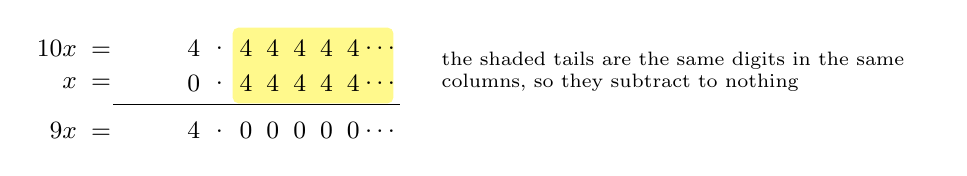
\begin{tikzpicture}[font=\small]
  \fill[yellow!45,rounded corners=2pt] \tailbox{0}{5}{-0.7}{0.26};
  \drow{0}{$10x\;=$}{$4$}{4,4,4,4,4,{$\ldots$}}
  \drow{-0.45}{$x\;=$}{$0$}{4,4,4,4,4,{$\ldots$}}
  \draw (-1.35,-0.72) -- (2.3,-0.72);
  \drow{-1.05}{$9x\;=$}{$4$}{0,0,0,0,0,{$\ldots$}}
  \node[anchor=west,font=\scriptsize,text width=6.2cm] at (2.7,-0.3)
    {the shaded tails are the same digits in the same columns, so they
     subtract to nothing};
\end{tikzpicture}
\end{center}
\ealpara{As caudas sombreadas são os mesmos \ealkeytr{algarismos} nas mesmas colunas, por isso subtraem até zero.}{the shaded tails are the same \ealkey{digits} in the same columns, so they subtract to nothing}
\vspace{-2pt}
\ealpara{Portanto $10x-x=4$, o que significa $9x=4$.}{So $10x-x=4$, which means $9x=4$.}

\smallskip
\ealpara{Passo 4 --- resolve. Temos $9$ lotes de $x$, por isso dividimos ambos os lados por $9$:}{Step 4 --- solve. We have $9$ lots of $x$, so we divide both sides by $9$:}

\vspace{-2pt}
\begin{center}
\divideboth{9x}{4}{x}{\dfrac{4}{9}}{9}
\end{center}
\end{wex}

\begin{enumerate}[resume]

\item \ealpara{Preenche as lacunas para converter $0.\dot{7}$ numa \ealkeytr{fração}.}{Fill in the gaps to turn $0.\dot{7}$ into a \ealkey{fraction}.}

\ealpara{Passo 1 --- introduz $x$. Escrevemos $x=0.\dot{7}$, portanto $x=0.7777\ldots$}{Step 1 --- introduce $x$. We write $x=0.\dot{7}$, so $x=0.7777\ldots$}

\smallskip
\ealpara{Passo 2 --- desloca os \ealkeytr{valores posicionais}. Multiplicar por $10$ desloca cada \ealkeytr{algarismo} uma casa para a esquerda: \newline $10x=7.7777\ldots$ (lembra-te de que $10x = 10 \times x$).}{Step 2 --- shift the \ealkey{place values}. Multiplying by $10$ moves every \ealkey{digit} one place to the left: \newline $10x=7.7777\ldots$ (remember $10x = 10 \times x$).}

\smallskip
\ealpara{Passo 3 --- subtrai. As duas caudas são idênticas, por isso cancelam-se quando subtraímos: $10x-x$.}{Step 3 --- subtract. The two tails are identical, so they cancel out when we subtract: $10x-x$.}

\begin{center}
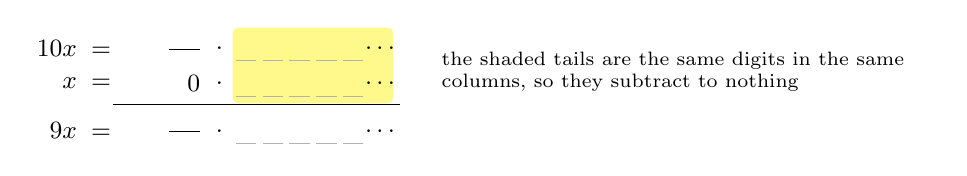
\begin{tikzpicture}[font=\small]
  \fill[yellow!45,rounded corners=2pt] \tailbox{0}{5}{-0.7}{0.26};
  \drowgap{0}{$10x\;=$}{\ansline[0.4cm]}{5}
  \drowgap{-0.45}{$x\;=$}{$0$}{5}
  \draw (-1.35,-0.72) -- (2.3,-0.72);
  \drowgap{-1.05}{$9x\;=$}{\ansline[0.4cm]}{5}
  \node[anchor=west,font=\scriptsize,text width=6.2cm] at (2.7,-0.3)
    {the shaded tails are the same digits in the same columns, so they
     subtract to nothing};
\end{tikzpicture}
\end{center}
\ealpara{As caudas sombreadas são os mesmos \ealkeytr{algarismos} nas mesmas colunas, por isso subtraem até zero.}{the shaded tails are the same \ealkey{digits} in the same columns, so they subtract to nothing}
\vspace{-2pt}
\ealpara{Portanto $10x-x=7$, o que significa $9x=7$.}{So $10x-x=7$, which means $9x=7$.}

\smallskip
\ealpara{Passo 4 --- resolve. Temos $9$ lotes de $x$, por isso dividimos ambos os lados por $9$. Apresenta os teus cálculos como no exemplo resolvido.}{Step 4 --- solve. We have $9$ lots of $x$, so we divide both sides by $9$. Set your working out like the worked example.}

\vspace{13em}

\newpage

\item \ealpara{Converte $0.\dot{8}$ numa \ealkeytr{fração}, usando os mesmos quatro passos.}{Turn $0.\dot{8}$ into a \ealkey{fraction}, using the same four steps.}
\ealpara{Passo 1 --- introduz $x$. Passo 2 --- desloca os \ealkeytr{valores posicionais}. Passo 3 --- subtrai. As duas caudas são idênticas, por isso cancelam-se quando subtraímos: $10x-x$. Portanto $10x-x=8$, o que significa $9x=8$. Passo 4 --- resolve. Divide ambos os lados por $9$.}{Step 1 --- introduce $x$. Step 2 --- shift the \ealkey{place values}. Step 3 --- subtract. The two tails are identical, so they cancel out when we subtract: $10x-x$. So $10x-x=8$, which means $9x=8$. Step 4 --- solve. Divide both sides by $9$.}
\begin{itemize}[label={},leftmargin=1.8em,itemsep=12pt,topsep=6pt]
  \item \textbf{Step 1 --- introduce $x$} \hfill \ansline[7cm]
  \item \textbf{Step 2 --- shift the \ealkey{place values}.} \hfill \ansline[7cm]
  \item \textbf{Step 3 --- subtract.} The two tails are identical, so they
        cancel out when we subtract: $10x-x$.
        \begin{center}
        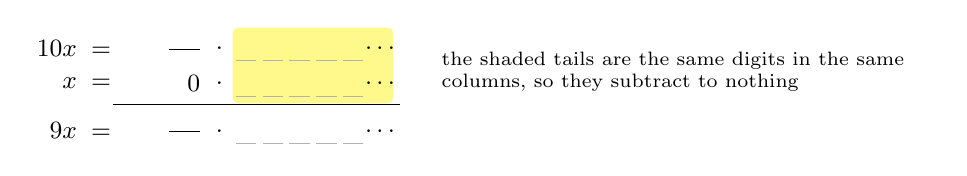
\begin{tikzpicture}[font=\small]
          \fill[yellow!45,rounded corners=2pt] \tailbox{0}{5}{-0.7}{0.26};
          \drowgap{0}{$10x\;=$}{\ansline[0.4cm]}{5}
          \drowgap{-0.45}{$x\;=$}{$0$}{5}
          \draw (-1.35,-0.72) -- (2.3,-0.72);
          \drowgap{-1.05}{$9x\;=$}{\ansline[0.4cm]}{5}
          \node[anchor=west,font=\scriptsize,text width=6.2cm] at (2.7,-0.3)
            {the shaded tails are the same digits in the same columns, so they
             subtract to nothing};
        \end{tikzpicture}
        \end{center}
        \vspace{-2pt}
        So $10x-x=\ansline[1.6cm]$, which means $9x=\ansline[1.6cm]$.
  \item \textbf{Step 4 --- solve.} Divide both sides by \ansline[0.9cm].

        \vspace{11em}
\end{itemize}

\item \ealpara{Converte cada um destes numa \ealkeytr{fração} na \ealkeytr{forma irredutível}. Escreve os quatro passos de cada vez.}{Turn each of these into a \ealkey{fraction} in its \ealkey{simplest form}. Write out all four steps each time.}
\begin{multicols}{4}
\begin{enumerate}
  \item $0.\dot{2}$
  \item $0.\dot{5}$
  \item $0.\dot{6}$
  \item $0.\dot{3}$
\end{enumerate}
\end{multicols}
\vspace{28em}

\end{enumerate}

\newpage

\parttitle{3}{Longer repeating blocks}

\ealpara{Tenta $0.\dot{3}\dot{6}$ da mesma maneira e as caudas não se cancelam. Multiplicar por $10$ desloca os \ealkeytr{valores posicionais} em uma casa, o que põe os dois \ealkeytr{algarismos} do bloco pela ordem errada. Um bloco de \emph{dois} \ealkeytr{algarismos} tem de ser deslocado em \emph{dois} \ealkeytr{valores posicionais}, por isso multiplicamos por $100$ em vez disso.}{Try $0.\dot{3}\dot{6}$ the same way and the tails do not cancel. Multiplying by $10$ shifts the \ealkey{place values} by one, which puts the two \ealkey{digits} of the block the wrong way round. A block of \emph{two} \ealkey{digits} has to be shifted by \emph{two} \ealkey{place values}, so we multiply by $100$ instead.}

\ealpara{As caudas diferem --- nada se cancela; as caudas coincidem --- estas cancelam-se.}{tails differ --- nothing cancels; tails match --- these cancel}

\vspace{4pt}
\begin{center}
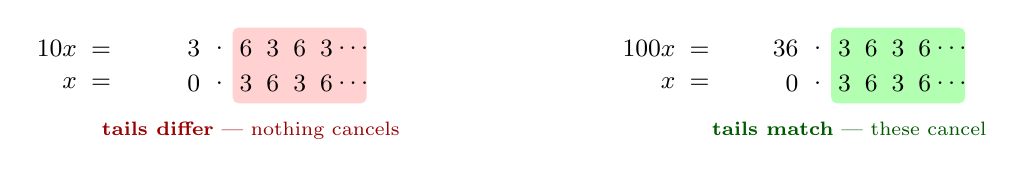
\begin{tikzpicture}[font=\small]
  \fill[red!18,rounded corners=2pt] \tailbox{0}{4}{-0.7}{0.26};
  \drow{0}{$10x\;=$}{$3$}{6,3,6,3,{$\ldots$}}
  \drow{-0.45}{$x\;=$}{$0$}{3,6,3,6,{$\ldots$}}
  \node[font=\scriptsize,anchor=north,red!60!black] at (0.4,-0.82)
    {\textbf{tails differ} --- nothing cancels};
  \begin{scope}[xshift=7.6cm]
    \fill[green!30,rounded corners=2pt] \tailbox{0}{4}{-0.7}{0.26};
    \drow{0}{$100x\;=$}{$36$}{3,6,3,6,{$\ldots$}}
    \drow{-0.45}{$x\;=$}{$0$}{3,6,3,6,{$\ldots$}}
    \node[font=\scriptsize,anchor=north,green!35!black] at (0.4,-0.82)
      {\textbf{tails match} --- these cancel};
  \end{scope}
\end{tikzpicture}
\end{center}
\vspace{4pt}

\ealpara{Converter $0.\dot{3}\dot{6}$ numa \ealkeytr{fração}}{turn $0.\dot{3}\dot{6}$ into a \ealkey{fraction}}
\begin{wex}{}
\small
\ealpara{Passo 1 --- introduz $x$: $x=0.\dot{3}\dot{6}$, portanto $x=0.363636\ldots$; Passo 2 --- desloca os \ealkeytr{valores posicionais}: $100x=36.363636\ldots$, o bloco tem $2$ \ealkeytr{algarismos} de comprimento; Passo 3 --- subtrai: $100x-x=36$, portanto $99x=36$; Passo 4 --- resolve: $x=\dfrac{36}{99}=\dfrac{4}{11}$.}{Step 1 --- introduce $x$: $x=0.\dot{3}\dot{6}$, so $x=0.363636\ldots$; Step 2 --- shift the \ealkey{place values}: $100x=36.363636\ldots$, the block is $2$ \ealkey{digits} long; Step 3 --- subtract: $100x-x=36$, so $99x=36$; Step 4 --- solve: $x=\dfrac{36}{99}=\dfrac{4}{11}$.}
\begin{tabular}{@{}ll@{\hspace{1.6em}}l@{}}
\textbf{Step 1 --- introduce $x$} & $x=0.\dot{3}\dot{6}$, so $x=0.363636\ldots$ & \\[8pt]
\textbf{Step 2 --- shift the \ealkey{place values}.} & $100x=36.363636\ldots$
  & the block is $2$ \ealkey{digits} long\\[8pt]
\textbf{Step 3 --- subtract.} & $100x-x=36$ & so $99x=36$\\[8pt]
\textbf{Step 4 --- solve.} & $x=\dfrac{36}{99}=\dfrac{4}{11}$ & \\
\end{tabular}
\end{wex}

\begin{enumerate}[resume]

\item \ealpara{Preenche as lacunas para converter $0.\dot{7}\dot{2}$ numa \ealkeytr{fração}.}{Fill in the gaps to turn $0.\dot{7}\dot{2}$ into a \ealkey{fraction}.}
\ealpara{Passo 1 --- introduz $x$: $x=0.727272\ldots$; Passo 2 --- desloca os \ealkeytr{valores posicionais}. O bloco tem um certo número de \ealkeytr{algarismos} de comprimento, portanto ...; Passo 3 --- subtrai; Passo 4 --- resolve.}{Step 1 --- introduce $x$: $x=0.727272\ldots$; Step 2 --- shift the \ealkey{place values}. The block is some \ealkey{digits} long, so ...; Step 3 --- subtract; Step 4 --- solve.}
\begin{itemize}[label={},leftmargin=1.8em,itemsep=12pt,topsep=6pt]
  \item \textbf{Step 1 --- introduce $x$} \hfill $x=0.727272\ldots$
  \item \textbf{Step 2 --- shift the \ealkey{place values}.} The block is
        \ansline[1cm] \ealkey{digits} long, so $\ansline[1cm]x=\ansline[2.2cm]$
  \item \textbf{Step 3 --- subtract.} \hfill $\ansline[1cm]x=\ansline[3cm]$
  \item \textbf{Step 4 --- solve.} \hfill $x=\ansline[3cm]$
\end{itemize}

\item \ealpara{Converte estes em \ealkeytr{frações} na \ealkeytr{forma irredutível}. A alínea (e) tem um bloco de três \ealkeytr{algarismos}, por isso pensa no que deves multiplicar.}{Turn these into \ealkey{fractions} in their \ealkey{simplest form}. Part (e) has a block of three \ealkey{digits}, so think about what to multiply by.}
\begin{multicols}{5}
\begin{enumerate}
  \item $0.\dot{1}\dot{5}$
  \item $0.\dot{0}\dot{6}$
  \item $0.\dot{5}\dot{4}$
  \item $0.\dot{9}\dot{0}$
  \item $0.\dot{1}0\dot{8}$
\end{enumerate}
\end{multicols}
\vspace{13em}

\newpage

\item
\begin{enumerate}
  \item \ealpara{Explica, por palavras tuas, como decides por que número multiplicar $x$.}{Explain, in your own words, how you decide what to multiply $x$ by.}

        \vspace{4em}
  \item \ealpara{Kayla converte $0.\dot{1}\dot{2}$ e obtém $\frac{12}{99}$. Ben converte o mesmo número e obtém $\frac{4}{33}$. Quem tem razão?}{Kayla converts $0.\dot{1}\dot{2}$ and gets $\frac{12}{99}$. Ben converts the same number and gets $\frac{4}{33}$. Who is right?}

        \vspace{5em}
\end{enumerate}

\end{enumerate}

\parttitle{4}{When the repeating part does not start straight away}

\ealpara{$0.1\dot{6}$ é mais difícil, porque o $1$ está na coluna das décimas e não se repete. Multiplicar por $10$ dá um número cuja cauda é toda seis, mas essa cauda não coincide com a cauda do próprio $x$. Em vez disso, deslocamos os \ealkeytr{valores posicionais} \emph{duas vezes} e subtraímos os dois resultados um do outro.}{$0.1\dot{6}$ is harder, because the $1$ is in the tenths column and does not repeat. Multiplying by $10$ gives a number whose tail is all sixes, but that tail does not match the tail of $x$ itself. Instead we shift the \ealkey{place values} \emph{twice}, and subtract the two results from each other.}

\ealpara{A cauda de $x$ começa com um $1$, por isso nunca coincidirá; estas duas coincidem, por isso subtrai estas duas.}{the tail of $x$ starts with a $1$, so it will never match; these two match, so subtract these two}

\vspace{2pt}
\begin{center}
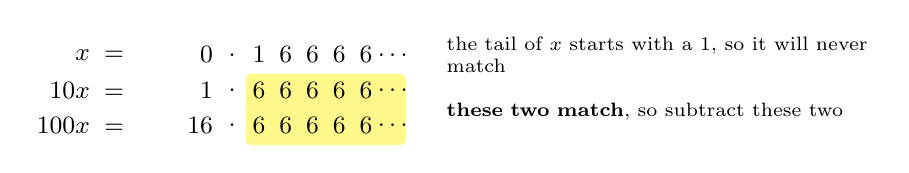
\begin{tikzpicture}[font=\small]
  \fill[yellow!45,rounded corners=2pt] \tailbox{0}{5}{-1.15}{-0.24};
  \drow{0}{$x\;=$}{$0$}{1,6,6,6,6,{$\ldots$}}
  \drow{-0.45}{$10x\;=$}{$1$}{6,6,6,6,6,{$\ldots$}}
  \drow{-0.9}{$100x\;=$}{$16$}{6,6,6,6,6,{$\ldots$}}
  \node[anchor=west,font=\scriptsize,text width=5.4cm] at (2.6,0)
    {the tail of $x$ starts with a $1$, so it will never match};
  \node[anchor=west,font=\scriptsize,text width=5.4cm] at (2.6,-0.72)
    {\textbf{these two match}, so subtract these two};
\end{tikzpicture}
\end{center}

\ealpara{Converter $0.1\dot{6}$ numa \ealkeytr{fração}}{turn $0.1\dot{6}$ into a \ealkey{fraction}}
\begin{wex}{}
\small
\ealpara{Passo 1 --- introduz $x$: $x=0.1\dot{6}$, portanto $x=0.16666\ldots$; Passo 2 --- desloca os \ealkeytr{valores posicionais}: $10x=1.6666\ldots$, desloca para além do $1$; $100x=16.6666\ldots$, desloca mais uma casa; Passo 3 --- subtrai: $100x-10x=16-1=15$, portanto $90x=15$; Passo 4 --- resolve: $x=\dfrac{15}{90}=\dfrac{1}{6}$.}{Step 1 --- introduce $x$: $x=0.1\dot{6}$, so $x=0.16666\ldots$; Step 2 --- shift the \ealkey{place values}: $10x=1.6666\ldots$, shift past the $1$; $100x=16.6666\ldots$, shift one more place; Step 3 --- subtract: $100x-10x=16-1=15$, so $90x=15$; Step 4 --- solve: $x=\dfrac{15}{90}=\dfrac{1}{6}$.}
\begin{tabular}{@{}ll@{\hspace{1.6em}}l@{}}
\textbf{Step 1 --- introduce $x$} & $x=0.1\dot{6}$, so $x=0.16666\ldots$ &\\[8pt]
\textbf{Step 2 --- shift the \ealkey{place values}.} & $10x=1.6666\ldots$
  & shift past the $1$\\[8pt]
 & $100x=16.6666\ldots$ & shift one more place\\[8pt]
\textbf{Step 3 --- subtract.} & $100x-10x=16-1=15$ & so $90x=15$\\[8pt]
\textbf{Step 4 --- solve.} & $x=\dfrac{15}{90}=\dfrac{1}{6}$ &\\
\end{tabular}
\end{wex}

\begin{enumerate}[resume]

\item \ealpara{Preenche as lacunas para converter $0.2\dot{7}$ numa \ealkeytr{fração}.}{Fill in the gaps to turn $0.2\dot{7}$ into a \ealkey{fraction}.}
\ealpara{Passo 1 --- introduz $x$: $x=0.27777\ldots$; Passo 2 --- desloca os \ealkeytr{valores posicionais}. Desloca para além do $2$; desloca mais uma casa; Passo 3 --- subtrai; portanto; Passo 4 --- resolve.}{Step 1 --- introduce $x$: $x=0.27777\ldots$; Step 2 --- shift the \ealkey{place values}. Shift past the $2$; shift one more place; Step 3 --- subtract; so; Step 4 --- solve.}
\begin{itemize}[label={},leftmargin=1.8em,itemsep=12pt,topsep=6pt]
  \item \textbf{Step 1 --- introduce $x$} \hfill $x=0.27777\ldots$
  \item \textbf{Step 2 --- shift the \ealkey{place values}.} Shift past the $2$:
        \hfill $10x=\ansline[3cm]$
  \item \hspace*{1.2em}Shift one more place: \hfill $100x=\ansline[3cm]$
  \item \textbf{Step 3 --- subtract.} \hfill $100x-10x=\ansline[3cm]$
  \item \hspace*{1.2em}so \hfill $90x=\ansline[3cm]$
  \item \textbf{Step 4 --- solve.} \hfill $x=\ansline[3cm]$
\end{itemize}

\newpage

\item \ealpara{Converte estes em \ealkeytr{frações} na \ealkeytr{forma irredutível}. Na alínea (d), o bloco que se repete tem dois \ealkeytr{algarismos} de comprimento, por isso pensa com cuidado em quais dois múltiplos de $x$ precisas.}{Turn these into \ealkey{fractions} in their \ealkey{simplest form}. In (d) the repeating block is two \ealkey{digits} long, so think carefully about which two multiples of $x$ you need.}
\begin{multicols}{4}
\begin{enumerate}
  \item $0.4\dot{3}$
  \item $0.58\dot{3}$
  \item $0.08\dot{3}$
  \item $0.1\dot{2}\dot{4}$
\end{enumerate}
\end{multicols}
\vspace{13em}

\item \ealpara{Os mesmos quatro passos funcionam quando o número é maior do que $1$. Converte estes em \ealkeytr{frações impróprias} na \ealkeytr{forma irredutível}.}{The same four steps work when the number is bigger than $1$. Turn these into \ealkey{improper fractions} in their \ealkey{simplest form}.}
\begin{multicols}{3}
\begin{enumerate}
  \item $2.\dot{7}$
  \item $1.\dot{4}\dot{5}$
  \item $3.\dot{1}\dot{8}$
\end{enumerate}
\end{multicols}
\vspace{13em}

\item \ealpara{\textbf{Prática mista.} Decide tu o que multiplicar de cada vez. Simplifica cada resposta.}{\textbf{Mixed practice.} Decide for yourself what to multiply by each time. Simplify every answer.}
\begin{multicols}{4}
\begin{enumerate}
  \item $0.\dot{8}$
  \item $0.\dot{6}\dot{3}$
  \item $0.2\dot{5}$
  \item $0.\dot{0}2\dot{7}$
  \item $0.7\dot{2}$
  \item $0.\dot{1}\dot{2}$
  \item $0.41\dot{6}$
  \item $0.06\dot{4}$
\end{enumerate}
\end{multicols}
\vspace{13em}

\end{enumerate}

\newpage

\parttitle{5}{Challenges}

\begin{enumerate}[resume]

\item \ealpara{O valor de $0.\dot{9}$.}{\textbf{The value of $0.\dot{9}$.}}
\begin{enumerate}
  \item \ealpara{Usa os quatro passos da Parte 2 em $x=0.\dot{9}$. Que \ealkeytr{fração} obténs?}{Use the four steps from Part 2 on $x=0.\dot{9}$. What \ealkey{fraction} do you get?}

        \vspace{12em}
  \item \ealpara{Ella diz: ``Isto tem de estar errado. $0.9999\ldots$ é obviamente um pouco menos do que $1$.'' A reta numérica abaixo marca $0.9$, depois $0.99$, depois $0.999$, e assim por diante. Usa-a, juntamente com o facto de que $\frac{1}{3}=0.\dot{3}$, para escreveres uma resposta à Ella.}{Ella says: ``That has to be wrong. $0.9999\ldots$ is obviously a bit less than $1$.'' The number line below marks $0.9$, then $0.99$, then $0.999$, and so on. Use it, together with the fact that $\frac{1}{3}=0.\dot{3}$, to write a reply to Ella.}
\end{enumerate}

\ealpara{Cada passo ao longo da reta fecha metade da lacuna que resta.}{each step along the line closes half of the gap that is left}

\vspace{4pt}
\begin{center}
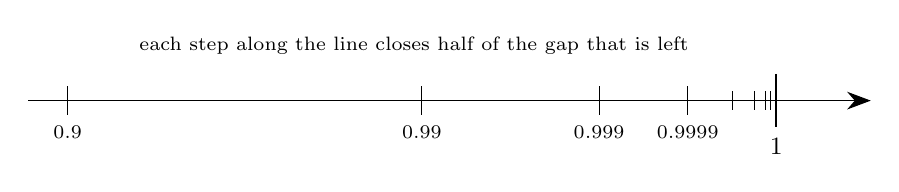
\begin{tikzpicture}[font=\small]
  \node[font=\scriptsize] at (4.4,0.7) {each step along the line closes half of the gap that is left};
  \draw[-{Stealth[length=3mm]}] (-0.5,0) -- (10.2,0);
  \foreach \x/\lab in {0/$0.9$, 4.5/$0.99$, 6.75/$0.999$, 7.875/$0.9999$}{
    \draw (\x,0.18) -- (\x,-0.18);
    \node[below,font=\scriptsize] at (\x,-0.2) {\lab};}
  \foreach \x in {8.44,8.72,8.86,8.93}{\draw (\x,0.12) -- (\x,-0.12);}
  \draw[thick] (9,0.34) -- (9,-0.34);
  \node[below,font=\small] at (9,-0.36) {$1$};
\end{tikzpicture}
\end{center}
\vspace{4pt}

\begin{enumerate}[resume]
  \item \ealpara{Qual é o maior número que é menor do que $1$? Explica.}{What is the largest number that is smaller than $1$? Explain.}

        \vspace{14em}
\end{enumerate}

\newpage

\item \ealpara{\textbf{Que \ealkeytr{frações} se repetem?} Algumas \ealkeytr{frações} dão decimais que terminam --- a estas chamamos \emph{\ealkeytr{dízimas finitas}} --- e outras dão decimais que se repetem para sempre.}{\textbf{Which \ealkey{fractions} recur?} Some \ealkey{fractions} give decimals that stop --- these are called \emph{\ealkey{terminating decimals}} --- and some give decimals that recur forever.}
\begin{enumerate}
  \item \ealpara{Completa a tabela usando a divisão curta. Circula as que terminam.}{Complete the table using short division. Circle the terminating ones.}

\vspace{3pt}
\begin{center}\small
\begin{tabular}{|c|c|c|c|c|c|}
\hline
\rule{0pt}{2.8em}$\frac{1}{2}=0.5$ & $\frac{1}{3}=$\rule{1.48cm}{0pt} &
$\frac{1}{4}=$\rule{1.48cm}{0pt} & $\frac{1}{5}=$\rule{1.48cm}{0pt} &
$\frac{1}{6}=$\rule{1.48cm}{0pt} & $\frac{1}{7}=$\rule{1.48cm}{0pt}\\
\hline
\rule{0pt}{2.8em}$\frac{1}{8}=$\rule{1.48cm}{0pt} & $\frac{1}{9}=$\rule{1.48cm}{0pt} &
$\frac{1}{10}=$\rule{1.48cm}{0pt} & $\frac{1}{11}=$\rule{1.48cm}{0pt} &
$\frac{1}{12}=$\rule{1.48cm}{0pt} & $\frac{1}{16}=$\rule{1.48cm}{0pt}\\
\hline
\end{tabular}
\end{center}
\vspace{3pt}

  \item \ealpara{Escreve cada \ealkeytr{denominador} que termina como um \ealkeytr{produto} dos seus \ealkeytr{fatores primos}. O que têm todos em comum?}{Write each terminating \ealkey{denominator} as a \ealkey{product} of its \ealkey{prime factors}. What do they all have in common?}

        \vspace{9em}
  \item \ealpara{Sem dividir, prevê se cada um destes termina ou se repete, e diz como sabes.}{Without dividing, predict whether each of these terminates or recurs, and say how you know.}
        \[\frac{1}{15}\qquad\frac{1}{40}\qquad\frac{1}{35}\qquad\frac{1}{64}\]

        \vspace{9em}
  \item \ealpara{Porque é que ter apenas $2$s e $5$s no \ealkeytr{denominador} faz a dízima parar? \emph{Sugestão: o que é especial em $2\times5$?}}{Why does having only $2$s and $5$s in the \ealkey{denominator} make the decimal stop? \emph{Hint: what is special about $2\times5$?}}

        \vspace{9em}
\end{enumerate}

\newpage

\item \ealpara{\textbf{Sétimos.} Um sétimo tem um bloco que se repete de seis \ealkeytr{algarismos}: $\dfrac{1}{7}=0.\dot{1}4285\dot{7}$.}{\textbf{Sevenths.} One seventh has a repeating block of six \ealkey{digits}: $\dfrac{1}{7}=0.\dot{1}4285\dot{7}$.}

\vspace{2pt}
\begin{minipage}[t]{0.58\linewidth}
\begin{enumerate}
  \item \ealpara{Usa a divisão curta para calcular $\frac{2}{7}$, $\frac{3}{7}$, $\frac{4}{7}$, $\frac{5}{7}$ e $\frac{6}{7}$ como \ealkeytr{dízimas periódicas}.}{Use short division to work out $\frac{2}{7}$, $\frac{3}{7}$, $\frac{4}{7}$, $\frac{5}{7}$ and $\frac{6}{7}$ as \ealkey{recurring decimals}.}

        \vspace{9em}
  \item \ealpara{O que reparas? Usa a roda para descrever o que acontece.}{What do you notice? Use the wheel to describe what happens.}

        \vspace{6em}
  \item \ealpara{Usa os quatro passos em $0.\dot{2}8571\dot{4}$ para o converter novamente numa \ealkeytr{fração} e verifica se está de acordo com a tua resposta à alínea (a).}{Use the four steps on $0.\dot{2}8571\dot{4}$ to turn it back into a \ealkey{fraction}, and check that it agrees with your answer to part (a).}

        \vspace{7em}
\end{enumerate}
\end{minipage}\hfill
\begin{minipage}[t]{0.38\linewidth}
\centering
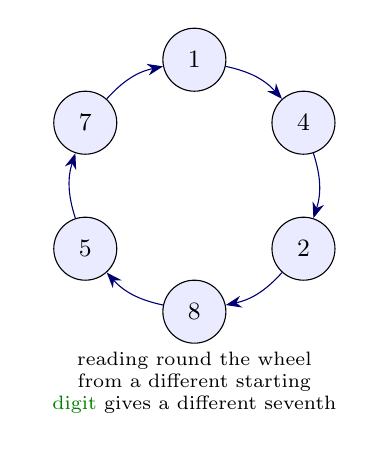
\begin{tikzpicture}[baseline=(current bounding box.north),font=\small]
  \foreach \d [count=\i from 0] in {1,4,2,8,5,7}{
    \node[circle,draw,minimum size=8mm,inner sep=0pt,fill=blue!8]
      (n\i) at ({90-\i*60}:1.6) {\d};}
  \foreach \i/\j in {0/1,1/2,2/3,3/4,4/5,5/0}{
    \draw[-{Stealth[length=2mm]},blue!45!black] (n\i) to[bend left=18] (n\j);}
  \node[font=\scriptsize,text width=4cm,align=center] at (0,-2.5)
    {reading round the wheel from a different starting \ealkey{digit} gives a
     different seventh};
\end{tikzpicture}
\end{minipage}

\ealpara{Ler à volta da roda a partir de um \ealkeytr{algarismo} inicial diferente dá um sétimo diferente.}{reading round the wheel from a different starting \ealkey{digit} gives a different seventh}

\newpage

\item \ealpara{\textbf{Faz os teus próprios.}}{\textbf{Make your own.}}
\begin{enumerate}
  \item \ealpara{Inventa uma \ealkeytr{dízima periódica} que se converta numa \ealkeytr{fração} com \ealkeytr{denominador} $11$. Mostra que funciona.}{Invent a \ealkey{recurring decimal} that converts to a \ealkey{fraction} with \ealkey{denominator} $11$. Show that it works.}

        \vspace{10em}
  \item \ealpara{Encontra a \ealkeytr{dízima periódica} que é exatamente $\frac{5}{6}$ e depois usa os quatro passos para a converter novamente em $\frac{5}{6}$.}{Find the \ealkey{recurring decimal} that is exactly $\frac{5}{6}$, then use the four steps to turn it back into $\frac{5}{6}$.}

        \vspace{10em}
  \item \ealpara{Será que \emph{todas} as \ealkeytr{dízimas periódicas} são iguais a uma \ealkeytr{fração}? Explica, por palavras tuas, porque é que a subtração funciona sempre, qualquer que seja a \ealkeytr{dízima periódica} com que começas.}{Is \emph{every} \ealkey{recurring decimal} equal to a \ealkey{fraction}? Explain, in your own words, why the subtraction always works, whatever \ealkey{recurring decimal} you start with.}

        \vspace{10em}
  \item \ealpara{Ben diz: ``$\pi=3.14159\ldots$ continua para sempre, por isso deve haver uma \ealkeytr{dízima periódica} que é exatamente igual a $\pi$.'' Usa a tua resposta à alínea (c) para explicar porque é que o Ben está errado.}{Ben says: ``$\pi=3.14159\ldots$ goes on forever, so there must be a \ealkey{recurring decimal} that is exactly equal to $\pi$.'' Use your answer to part (c) to explain why Ben is wrong.}

        \vspace{10em}
\end{enumerate}

\end{enumerate}

\newpage

\heading{Answers}

{\small
\begin{multicols}{2}
\raggedcolumns
\setlength{\parskip}{4pt}

\textbf{Q1.} (a) $0.55555555$ \quad (b) $0.18181818$ \quad (c) $0.37777777$
\quad (d) $0.20620620$ \quad (e) $0.45151515$ \quad (f) $0.99999999$

\textbf{Q2.} (a) $0.\dot{8}$ \quad (b) $0.\dot{6}\dot{3}$ \quad
(c) $0.2\dot{4}$ \quad (d) $0.\dot{1}5\dot{7}$ \quad (e) $0.91\dot{6}$ \quad
(f) $0.4\dot{0}\dot{5}$

\ealpara{\textbf{Q3.} (a) $0.\dot{4}\dot{5}=0.454545$ e $0.4\dot{5}=0.455555$, portanto $0.4\dot{5}$ é maior --- coincidem até duas \ealkeytr{casas decimais}, mas o terceiro \ealkeytr{algarismo} é $5$ contra $4$. \quad (b) Muitas respostas, por exemplo $0.\dot{3}\dot{5}=0.353535\ldots$}{\textbf{Q3.} (a) $0.\dot{4}\dot{5}=0.454545$ and $0.4\dot{5}=0.455555$, so $0.4\dot{5}$ is bigger --- they agree to two \ealkey{decimal places}, but the third \ealkey{digit} is $5$ against $4$. \quad (b) Many answers, for example $0.\dot{3}\dot{5}=0.353535\ldots$}

\textbf{Q4.} $10x=7.7777\ldots$; \; $10x-x=7$; \; $9x=7$; \;
$x=\tfrac{7}{9}$

\textbf{Q5.} $x=0.8888\ldots$; \; $10x=8.8888\ldots$; \;
$10x-x=8$, so $9x=8$; \; $x=\tfrac{8}{9}$

\textbf{Q6.} (a) $\tfrac{2}{9}$ \quad (b) $\tfrac{5}{9}$ \quad
(c) $\tfrac{6}{9}=\tfrac{2}{3}$ \quad (d) $\tfrac{3}{9}=\tfrac{1}{3}$

\ealpara{\textbf{Q7.} O bloco tem $2$ \ealkeytr{algarismos} de comprimento, por isso multiplica por $100$: $100x=72.727272\ldots$; \; $99x=72$; \; $x=\tfrac{72}{99}=\tfrac{8}{11}$}{\textbf{Q7.} The block is $2$ \ealkey{digits} long, so multiply by $100$: $100x=72.727272\ldots$; \; $99x=72$; \; $x=\tfrac{72}{99}=\tfrac{8}{11}$}

\ealpara{\textbf{Q8.} (a) $\tfrac{15}{99}=\tfrac{5}{33}$ \quad (b) $\tfrac{6}{99}=\tfrac{2}{33}$ \quad (c) $\tfrac{54}{99}=\tfrac{6}{11}$ \quad (d) $\tfrac{90}{99}=\tfrac{10}{11}$ \quad (e) $\tfrac{108}{999}=\tfrac{4}{37}$, multiplicando por $1000$}{\textbf{Q8.} (a) $\tfrac{15}{99}=\tfrac{5}{33}$ \quad (b) $\tfrac{6}{99}=\tfrac{2}{33}$ \quad (c) $\tfrac{54}{99}=\tfrac{6}{11}$ \quad (d) $\tfrac{90}{99}=\tfrac{10}{11}$ \quad (e) $\tfrac{108}{999}=\tfrac{4}{37}$, multiplying by $1000$}

\ealpara{\textbf{Q9.} (a) Conta os \ealkeytr{algarismos} no bloco que se repete. Se houver $n$ deles, multiplica por $1$ seguido de $n$ zeros, para que o bloco se desloque um número inteiro de vezes e as caudas voltem a alinhar-se. \quad (b) Ambos têm razão: $\tfrac{12}{99}=\tfrac{4}{33}$. Ben simplificou a dele, que é o que a pergunta pede.}{\textbf{Q9.} (a) Count the \ealkey{digits} in the repeating block. If there are $n$ of them, multiply by $1$ followed by $n$ zeros, so that the block shifts a whole number of times and the tails line up again. \quad (b) Both are right: $\tfrac{12}{99}=\tfrac{4}{33}$. Ben has simplified his, which is what the question asks for.}

\textbf{Q10.} $10x=2.7777\ldots$; \; $100x=27.7777\ldots$; \;
$100x-10x=27-2=25$; \; $90x=25$; \; $x=\tfrac{25}{90}=\tfrac{5}{18}$

\ealpara{\textbf{Q11.} (a) $\tfrac{39}{90}=\tfrac{13}{30}$ \quad (b) $\tfrac{525}{900}=\tfrac{7}{12}$ \quad (c) $\tfrac{75}{900}=\tfrac{1}{12}$ \quad (d) $\tfrac{123}{990}=\tfrac{41}{330}$, usando $1000x-10x$}{\textbf{Q11.} (a) $\tfrac{39}{90}=\tfrac{13}{30}$ \quad (b) $\tfrac{525}{900}=\tfrac{7}{12}$ \quad (c) $\tfrac{75}{900}=\tfrac{1}{12}$ \quad (d) $\tfrac{123}{990}=\tfrac{41}{330}$, using $1000x-10x$}

\textbf{Q12.} (a) $\tfrac{25}{9}$ \quad (b) $\tfrac{144}{99}=\tfrac{16}{11}$
\quad (c) $\tfrac{315}{99}=\tfrac{35}{11}$

\textbf{Q13.} (a) $\tfrac{8}{9}$ \quad (b) $\tfrac{63}{99}=\tfrac{7}{11}$
\quad (c) $\tfrac{23}{90}$ \quad (d) $\tfrac{27}{999}=\tfrac{1}{37}$ \quad
(e) $\tfrac{65}{90}=\tfrac{13}{18}$ \quad (f) $\tfrac{12}{99}=\tfrac{4}{33}$
\quad (g) $\tfrac{375}{900}=\tfrac{5}{12}$ \quad
(h) $\tfrac{58}{900}=\tfrac{29}{450}$

\ealpara{\textbf{Q14.} (a) $10x=9.9999\ldots$, portanto $9x=9$ e $x=\tfrac{9}{9}=1$. \quad (b) O método é sólido, por isso $0.\dot{9}$ é realmente $1$. Cada passo ao longo da reta numérica fecha metade do que resta, por isso as marcas aproximam-se de $1$ tanto quanto quiseres --- não há espaço entre $0.\dot{9}$ e $1$ para serem números diferentes. Além disso, $\frac{1}{3}=0.\dot{3}$, e multiplicar ambos os lados por $3$ dá $1=0.\dot{9}$. \quad (c) Não existe. Qualquer número que nomeies abaixo de $1$, há sempre outro número entre ele e $1$ --- que é exatamente a razão pela qual $0.\dot{9}$ tem de \emph{ser} $1$ em vez de ficar logo abaixo dele.}{\textbf{Q14.} (a) $10x=9.9999\ldots$, so $9x=9$ and $x=\tfrac{9}{9}=1$. \quad (b) The method is sound, so $0.\dot{9}$ really is $1$. Every step along the number line closes half of what is left, so the marks get as close to $1$ as you like --- there is no room left between $0.\dot{9}$ and $1$ for them to be different numbers. Also $\frac{1}{3}=0.\dot{3}$, and multiplying both sides by $3$ gives $1=0.\dot{9}$. \quad (c) There isn't one. Whatever number you name below $1$, there is always another number between it and $1$ --- which is exactly why $0.\dot{9}$ has to \emph{be} $1$ rather than sit just below it.}

\ealpara{\textbf{Q15.} (a) $\tfrac{1}{3}=0.\dot{3}$, $\tfrac{1}{4}=0.25$, $\tfrac{1}{5}=0.2$, $\tfrac{1}{6}=0.1\dot{6}$, $\tfrac{1}{7}=0.\dot{1}4285\dot{7}$, $\tfrac{1}{8}=0.125$, $\tfrac{1}{9}=0.\dot{1}$, $\tfrac{1}{10}=0.1$, $\tfrac{1}{11}=0.\dot{0}\dot{9}$, $\tfrac{1}{12}=0.08\dot{3}$, $\tfrac{1}{16}=0.0625$. As que terminam são $\tfrac{1}{2},\tfrac{1}{4},\tfrac{1}{5},\tfrac{1}{8},\tfrac{1}{10},\tfrac{1}{16}$. \quad (b) $2$, $2^2$, $5$, $2^3$, $2\times5$, $2^4$ --- cada um é construído apenas com $2$s e $5$s. \quad (c) $\tfrac{1}{15}$ repete-se, porque $15=3\times5$ e o $3$ não é permitido; $\tfrac{1}{40}$ termina, porque $40=2^3\times5$; $\tfrac{1}{35}$ repete-se, porque $35=5\times7$; $\tfrac{1}{64}$ termina, porque $64=2^6$. \quad (d) Uma \ealkeytr{dízima finita} é apenas uma \ealkeytr{fração} sobre $10$, $100$, $1000$, \ldots, e $10=2\times5$. Portanto, uma \ealkeytr{fração} pode ser reescrita sobre uma \ealkeytr{potência} de dez exatamente quando o seu \ealkeytr{denominador} é construído com $2$s e $5$s; qualquer outro \ealkeytr{fator primo} nunca pode ser cancelado.}{\textbf{Q15.} (a) $\tfrac{1}{3}=0.\dot{3}$, $\tfrac{1}{4}=0.25$, $\tfrac{1}{5}=0.2$, $\tfrac{1}{6}=0.1\dot{6}$, $\tfrac{1}{7}=0.\dot{1}4285\dot{7}$, $\tfrac{1}{8}=0.125$, $\tfrac{1}{9}=0.\dot{1}$, $\tfrac{1}{10}=0.1$, $\tfrac{1}{11}=0.\dot{0}\dot{9}$, $\tfrac{1}{12}=0.08\dot{3}$, $\tfrac{1}{16}=0.0625$. The terminating ones are $\tfrac{1}{2},\tfrac{1}{4},\tfrac{1}{5},\tfrac{1}{8},\tfrac{1}{10},\tfrac{1}{16}$. \quad (b) $2$, $2^2$, $5$, $2^3$, $2\times5$, $2^4$ --- every one is built out of $2$s and $5$s only. \quad (c) $\tfrac{1}{15}$ recurs, since $15=3\times5$ and the $3$ is not allowed; $\tfrac{1}{40}$ terminates, since $40=2^3\times5$; $\tfrac{1}{35}$ recurs, since $35=5\times7$; $\tfrac{1}{64}$ terminates, since $64=2^6$. \quad (d) A \ealkey{terminating decimal} is just a \ealkey{fraction} over $10$, $100$, $1000$, \ldots, and $10=2\times5$. So a \ealkey{fraction} can be rewritten over a \ealkey{power} of ten exactly when its \ealkey{denominator} is built from $2$s and $5$s; any other \ealkey{prime factor} can never be cancelled away.}

\ealpara{\textbf{Q16.} (a) $\tfrac{2}{7}=0.\dot{2}8571\dot{4}$, $\tfrac{3}{7}=0.\dot{4}2857\dot{1}$, $\tfrac{4}{7}=0.\dot{5}7142\dot{8}$, $\tfrac{5}{7}=0.\dot{7}1428\dot{5}$, $\tfrac{6}{7}=0.\dot{8}5714\dot{2}$. \quad (b) Todos usam os mesmos seis \ealkeytr{algarismos} na mesma ordem cíclica, $1\to4\to2\to8\to5\to7\to1$; cada sétimo começa simplesmente num lugar diferente da roda. \quad (c) O bloco tem $6$ \ealkeytr{algarismos} de comprimento, por isso multiplica por $1\,000\,000$: isto dá $999\,999x=285\,714$, portanto $x=\tfrac{285714}{999999}=\tfrac{2}{7}$, dividindo o de cima e o de baixo por $142\,857$.}{\textbf{Q16.} (a) $\tfrac{2}{7}=0.\dot{2}8571\dot{4}$, $\tfrac{3}{7}=0.\dot{4}2857\dot{1}$, $\tfrac{4}{7}=0.\dot{5}7142\dot{8}$, $\tfrac{5}{7}=0.\dot{7}1428\dot{5}$, $\tfrac{6}{7}=0.\dot{8}5714\dot{2}$. \quad (b) They all use the same six \ealkey{digits} in the same cyclic order, $1\to4\to2\to8\to5\to7\to1$; each seventh simply starts at a different place on the wheel. \quad (c) The block is $6$ \ealkey{digits} long, so multiply by $1\,000\,000$: this gives $999\,999x=285\,714$, so $x=\tfrac{285714}{999999}=\tfrac{2}{7}$, dividing top and bottom by $142\,857$.}

\ealpara{\textbf{Q17.} (a) Muitas respostas. Por exemplo, $0.\dot{2}\dot{7}$ dá $99x=27$, portanto $x=\tfrac{27}{99}=\tfrac{3}{11}$; serve qualquer bloco de dois \ealkeytr{algarismos} que seja múltiplo de $9$ mas não de $11$. \quad (b) $\tfrac{5}{6}=0.8\dot{3}$, e verificando: $100x-10x=83-8=75$, portanto $90x=75$ e $x=\tfrac{75}{90}=\tfrac{5}{6}$. \quad (c) Sim. Qualquer que seja o decimal, deslocá-lo pelo comprimento do bloco que se repete produz sempre um segundo número com uma cauda idêntica, por isso a subtração deixa sempre um número inteiro. Isso dá uma \ealkeytr{equação} da forma (número inteiro)$\,\times x=$ (número inteiro), e dividir dá uma \ealkeytr{fração}. \quad (d) $\pi$ não é uma \ealkeytr{fração}, e a alínea (c) mostra que todas as \ealkeytr{dízimas periódicas} são uma. Portanto, nenhuma \ealkeytr{dízima periódica} pode ser igual a $\pi$: os seus \ealkeytr{algarismos} continuam para sempre sem nunca se fixarem num bloco que se repete.}{\textbf{Q17.} (a) Many answers. For example $0.\dot{2}\dot{7}$ gives $99x=27$, so $x=\tfrac{27}{99}=\tfrac{3}{11}$; any two-\ealkey{digit} block that is a multiple of $9$ but not of $11$ will do. \quad (b) $\tfrac{5}{6}=0.8\dot{3}$, and checking: $100x-10x=83-8=75$, so $90x=75$ and $x=\tfrac{75}{90}=\tfrac{5}{6}$. \quad (c) Yes. Whatever the decimal, shifting it by the length of the repeating block always produces a second number with an identical tail, so the subtraction always leaves a whole number. That gives an \ealkey{equation} of the form (whole number)$\,\times x=$ (whole number), and dividing gives a \ealkey{fraction}. \quad (d) $\pi$ is not a \ealkey{fraction}, and part (c) shows that every \ealkey{recurring decimal} is one. So no \ealkey{recurring decimal} can equal $\pi$: its \ealkey{digits} go on forever without ever settling into a repeating block.}

\end{multicols}
}

\end{document}